\documentclass[12pt,aspectratio=169]{beamer}
% Shared Beamer setup for BIM Resilience biological-simulations decks.
% \input{} after \documentclass{beamer}.

\usetheme{Madrid}
\setbeamertemplate{navigation symbols}{}

\usepackage[T1]{fontenc}
\usepackage[utf8]{inputenc}
\usepackage{lmodern}
\usepackage{graphicx}
\usepackage{booktabs}
\usepackage{tikz}
\usetikzlibrary{arrows.meta,positioning,shapes.geometric,calc}
\usepackage{enumitem}
\setlist[itemize,1]{itemsep=2pt,topsep=2pt,parsep=0pt,partopsep=0pt,leftmargin=1.6em,label=\usebeamertemplate{itemize item}}
\setlist[itemize,2]{itemsep=1pt,topsep=1pt,parsep=0pt,partopsep=0pt,leftmargin=1.4em,label=\usebeamertemplate{itemize subitem}}
\setbeamerfont{normal text}{size=\normalsize}
\setbeamerfont{itemize/enumerate body}{size=\small}
\setbeamerfont{itemize/enumerate subbody}{size=\footnotesize}
\setbeamerfont{frametitle}{size=\Large,series=\bfseries}
\setbeamerfont{caption}{size=\footnotesize}
\usepackage{hyperref}
\hypersetup{colorlinks=true,linkcolor=,urlcolor=blue,citecolor=blue}

\definecolor{bimnavy}{HTML}{0F2A44}
\definecolor{bimnavylight}{HTML}{1B3A5C}
\definecolor{bimorange}{HTML}{C0410A}
\definecolor{bimsteel}{HTML}{4A7A9B}
\definecolor{bimcarry}{HTML}{0072B2}
\definecolor{bimreduce}{HTML}{E69F00}

\setbeamercolor{palette primary}{bg=bimnavy,fg=white}
\setbeamercolor{palette secondary}{bg=bimnavylight,fg=white}
\setbeamercolor{palette tertiary}{bg=bimsteel,fg=white}
\setbeamercolor{palette quaternary}{bg=bimnavy,fg=white}
\setbeamercolor{structure}{fg=bimorange}
\setbeamercolor{normal text}{fg=black,bg=white}
\setbeamercolor{background canvas}{bg=white}
\setbeamercolor{frametitle}{fg=white,bg=bimnavy}
\setbeamercolor{title}{fg=white,bg=bimnavy}
\setbeamercolor{section in head/foot}{fg=white,bg=bimnavy}
\setbeamercolor{subsection in head/foot}{fg=white,bg=bimsteel}
\setbeamercolor{author in head/foot}{fg=white,bg=bimnavy}
\setbeamercolor{title in head/foot}{fg=white,bg=bimnavy}
\setbeamercolor{date in head/foot}{fg=white,bg=bimnavy}
\setbeamercolor{page number in head/foot}{fg=bimnavy}
\setbeamercolor{block title}{fg=white,bg=bimorange}
\setbeamercolor{block body}{fg=black,bg=bimorange!8}
\setbeamercolor{item}{fg=bimorange}
\setbeamercolor{itemize item}{fg=bimorange}
\setbeamercolor{itemize subitem}{fg=bimsteel}
\setbeamercolor{alerted text}{fg=bimorange}
\setbeamertemplate{footline}[frame number]

\graphicspath{{./}}
\newcommand{\beamfig}[1]{%
  \includegraphics[width=\linewidth,height=0.58\textheight,keepaspectratio]{#1}}
\newcommand{\beamfigbig}[1]{%
  \includegraphics[width=\linewidth,height=0.74\textheight,keepaspectratio]{#1}}
\newcommand{\figcap}[1]{{\footnotesize\textcolor{bimsteel}{#1}}}

% Title slide: optional second argument is an orange eyebrow (e.g. ``10 minutes'').
\newcommand{\bimtitleslide}[2][]{%
  \begin{frame}[plain]
    \begin{tikzpicture}[remember picture, overlay]
      \fill[bimnavy] (current page.south west) rectangle (current page.north east);
      \node[regular polygon, regular polygon sides=6, minimum size=2.6cm,
            fill=bimorange, fill opacity=0.35, anchor=center, rotate=10]
        at ($(current page.south east)+(-1.6cm,1.3cm)$) {};
      \node[regular polygon, regular polygon sides=6, minimum size=2.0cm,
            fill=bimsteel, fill opacity=0.45, anchor=center, rotate=10]
        at ($(current page.south east)+(-3.4cm,2.1cm)$) {};
      \node[regular polygon, regular polygon sides=6, minimum size=1.4cm,
            fill=bimsteel, fill opacity=0.3, anchor=center, rotate=10]
        at ($(current page.south east)+(-1.0cm,3.1cm)$) {};
      \draw[bimorange, line width=2.4pt]
        ($(current page.west)+(2.1cm,1.9cm)$) -- ++(0,-3.3cm);
      \if\relax\detokenize{#1}\relax\else
        \node[anchor=west, font=\small\bfseries, text=bimorange!90!white]
          at ($(current page.west)+(2.7cm,1.55cm)$) {#1};
      \fi
      \node[anchor=west, text width=10.8cm, align=left, font=\Huge\bfseries, text=white]
        at ($(current page.west)+(2.7cm,1.05cm)$) {Biological Simulations};
      \node[anchor=west, text width=10.8cm, align=left, font=\Large, text=white]
        at ($(current page.west)+(2.7cm,0.35cm)$) {Stocks, Advice, and Scenarios};
      \node[anchor=west, text width=10.4cm, align=left, font=\normalsize, text=bimorange!85!white]
        at ($(current page.west)+(2.7cm,-0.5cm)$) {#2};
      \node[anchor=west, font=\small, text=white!85!bimnavy]
        at ($(current page.west)+(2.7cm,-1.75cm)$)
        {Laurence T. Kell \quad\textbullet\quad BIM Resilience Project \quad\textbullet\quad \today};
    \end{tikzpicture}
  \end{frame}}


\title[BIM Resilience --- full]{Biological Simulations: Stocks, Advice, and Scenarios}
\subtitle{Full deck --- from biological advice and ``what ifs'' to industry resilience via CREST}
\author{Laurence T. Kell}
\institute{BIM Resilience Project}
\date{\today}

\begin{document}

\bimtitleslide[Full deck]{From biological advice and ``what ifs'' to industry resilience via CREST}

% ------------------------------------------------------------
\begin{frame}{Outline}
  \begin{itemize}
    \item \textbf{1.\ Advice} --- mainly conditioned on the \emph{past}
    \item \textbf{2.\ Resilience} --- depends on the \emph{future}, ``what ifs'', and does it matter?
    \item \textbf{3.\ Mackerel} --- examples: recruitment, random variability, $M$ shock
    \item \textbf{4.\ CREST} --- fleet outcomes, from diagnosis to prognosis
  \end{itemize}
  \vspace{4mm}
  {\footnotesize\textcolor{bimsteel}{Resilience means being ready --- the future will not be like the past.}}
\end{frame}


\begin{frame}{Resilience in a Changing World}
	\footnotesize
	\begin{itemize}
		\item \textbf{Can't Bounce Back} --- productivity and hence reference points are \emph{changing}
		\item \textbf{Stay Viable} --- not restore an equilibrium
	\end{itemize}
	\vspace{2mm}
	\begin{columns}[T]
		\begin{column}{0.48\textwidth}
			\textbf{Why it matters}
			\begin{itemize}
				\item Past strategies can fail under new regimes
				\item Fisheries: shifting productivity, distribution, recruitment, ...
			\end{itemize}
		\end{column}
		\begin{column}{0.48\textwidth}
			\textbf{What resilience means}
			\begin{itemize}
				\item \textbf{Persist} --- keep functioning
				\item \textbf{Adapt} --- change with conditions
				\item \textbf{Transform} --- change the system when needed
			\end{itemize}
		\end{column}
	\end{columns}
\end{frame}

% ============================================================
\section{Advice}

\begin{frame}{1. Advice --- annual updates}
  \begin{columns}[T]
    \begin{column}{0.32\textwidth}
      \footnotesize
      \textbf{Update}: advice is based on
      \vspace{1mm}
      \begin{itemize}
        \item Adding last year's catches and surveys, then re-running the model
        \item Series extends one year; structure and reference points stay the same
        \item Terminal year moves
      \end{itemize}
    \end{column}
    \begin{column}{0.64\textwidth}
      \centering
      \beamfigbig{fig1.png}\\
      \figcap{SSB by stock --- update peels 2016--2021}
    \end{column}
  \end{columns}
\end{frame}

\begin{frame}{1. Advice --- benchmarks change the story}
  \begin{columns}[T]
    \begin{column}{0.32\textwidth}
      \footnotesize
      \textbf{Benchmark}: periodic reset
      \vspace{1mm}
      \begin{itemize}
        \item Full peer review of assumptions, data and reference points
        \item $B_{\mathrm{trigger}}$, $B_{\mathrm{lim}}$ and $F_{\mathrm{MSY}}$ change
        \item Productivity regimes change them further
        \item \textbf{Resilience}: even the past may change
      \end{itemize}
    \end{column}
    \begin{column}{0.64\textwidth}
      \centering
      \beamfigbig{fig2.png}\\
      \figcap{SSB by stock --- assessment years 2016--2026}
    \end{column}
  \end{columns}
\end{frame}

\begin{frame}{1. Advice --- status relative to $B_{\mathrm{trigger}}$}
  \begin{columns}[T]
    \begin{column}{0.32\textwidth}
      \footnotesize
      Management is relative to reference points:
      \vspace{1mm}
      \begin{itemize}
        \item $\mathrm{SSB}/B_{\mathrm{trigger}}=1$
        \begin{itemize}
          \item \textcolor{bimcarry}{$> 1$ --- carry on}
          \item \textcolor{bimreduce}{$<{ }1$ --- reduce $F$, catch and effort}
        \end{itemize}
        \item Crossing the threshold flips status and advice
        \item Benchmark can change $B_{\mathrm{trigger}}$ and flip the story
      \end{itemize}
    \end{column}
    \begin{column}{0.64\textwidth}
      \centering
      \beamfigbig{fig3.png}\\
      \figcap{$\mathrm{SSB}/B_{\mathrm{trigger}}$ --- blue above 1, orange below}
    \end{column}
  \end{columns}
\end{frame}

% ============================================================
\section{Scenarios}

\begin{frame}{2. Scenarios --- what ifs}
  Examples
  \begin{itemize}
    \item Projections under \textbf{fixed} fishing effort, or MSE for ICES AR
    \item Common questions:
      \begin{itemize}
        \item Status-quo $F$ with recent productivity
        \item Same $F$ with poorer recruitment ($75\%$, $50\%$)
        \item $F_{\mathrm{MSY}}$ for recent recruitment \emph{regime}
      \end{itemize}
  \end{itemize}
\end{frame}

\begin{frame}{2. Scenarios --- pelagics}
  \begin{columns}[T]
    \begin{column}{0.46\textwidth}
      \textbf{Pelagics}: boarfish, western horse mackerel, NEA mackerel, blue whiting
      \begin{itemize}
        \item Status-quo, recruitment regimes
        \item \textbf{Resilience}: under current fishing, does catch get better, stay the same, or get worse?
      \end{itemize}
    \end{column}
    \begin{column}{0.5\textwidth}
      \centering
      \beamfig{fig4.png}\\
      \figcap{Projected catch by scenario}
    \end{column}
  \end{columns}
\end{frame}

\begin{frame}{2. Scenarios --- demersal}
  \begin{columns}[T]
    \begin{column}{0.46\textwidth}
      \textbf{Demersal}: anglerfishes, northern hake, megrims, whitings
      \begin{itemize}
        \item Status-quo, recruitment regimes
        \item \textbf{Resilience}: under current fishing, does catch get better, stay the same, or get worse?
      \end{itemize}
    \end{column}
    \begin{column}{0.5\textwidth}
      \centering
      \beamfig{fig5.png}\\
      \figcap{Projected catch by scenario}
    \end{column}
  \end{columns}
\end{frame}

\begin{frame}{2. Scenarios --- Nephrops}
  \begin{columns}[T]
    \begin{column}{0.46\textwidth}
      \textbf{Nephrops}: functional units OMs (JABBA / biodyn)
      \begin{itemize}
        \item \textbf{Scenarios}:
          \begin{itemize}
            \item Status-quo harvest; same harvest with process error $\times 0.75$ / $0.50$
            \item \textbf{Resilience}: spatial squeeze, effort $\neq F$?
          \end{itemize}
      \end{itemize}
    \end{column}
    \begin{column}{0.5\textwidth}
      \centering
      \beamfig{fig6.png}\\
      \figcap{Projected catch by scenario}
    \end{column}
  \end{columns}
\end{frame}

% ============================================================
\section{Mackerel worked example}

\begin{frame}{3. Mackerel --- example}
  \textbf{``What if''} based on current $F$
  \begin{itemize}
    \item Stresses
      \begin{itemize}
        \item Lower recruitment (productivity)
        \item One-off natural-mortality shock (a flip, not a trend)
        \item Year-to-year recruitment noise (the spread fleets live with)
      \end{itemize}
    \item Biological trajectories are what CREST carries through to fleet values and effort
  \end{itemize}
\end{frame}

\begin{frame}{3. Mackerel --- recruitment levels}
  \begin{columns}[T]
    \begin{column}{0.46\textwidth}
      \begin{itemize}
        \item Fixed status-quo $F$
        \item Recruitment deviance scaled relative to the recent residual mean:
          \begin{itemize}
            \item $\times 1$, $\times 0.75$, $\times 0.5$, $\times 0.25$
          \end{itemize}
        \item Question: if effort stays as now, how far does catch fall when productivity is poorer?
      \end{itemize}
    \end{column}
    \begin{column}{0.5\textwidth}
      \centering
      \beamfig{fig_mac_rec.png}\\
      \figcap{Catch under recruitment multipliers}
    \end{column}
  \end{columns}
\end{frame}

\begin{frame}{3. Mackerel --- one-off $M$ shock}
  \begin{columns}[T]
    \begin{column}{0.46\textwidth}
      \begin{itemize}
        \item Same status-quo $F$ and baseline recruitment deviance
        \item \textbf{Shock}: natural mortality $\times 5$ for a single year (2035), then back to baseline $M$
        \item A pulse --- the kind of flip a smooth forecast misses
        \item Compare shocked catch path with the no-shock baseline
      \end{itemize}
    \end{column}
    \begin{column}{0.5\textwidth}
      \centering
      \beamfig{fig_mac_mshock.png}\\
      \figcap{Catch: baseline vs $M\times 5$ in 2035}
    \end{column}
  \end{columns}
\end{frame}

\begin{frame}{3. Mackerel --- random recruitment}
  \begin{columns}[T]
    \begin{column}{0.46\textwidth}
      \begin{itemize}
        \item Year-to-year noise around recent recruitment
        \item Recent $F$
        \item Ribbon = 5--95\% of \textbf{catch} paths; black = one example year sequence
        \item \textbf{Resilience}: what fleets have to live with --- not a mean trend
      \end{itemize}
    \end{column}
    \begin{column}{0.5\textwidth}
      \centering
      \beamfig{fig_mac_rand.png}\\
      \figcap{Stochastic catch: median, band, example path}
    \end{column}
  \end{columns}
\end{frame}

% ============================================================
\section{CREST}

\begin{frame}{4. CREST --- not an answering machine}
  \begin{columns}[T]
    \begin{column}{0.52\textwidth}
      \textbf{CREST}: Capacity, Resilience and Economic Shock Transmission
      \vspace{2mm}
      \begin{itemize}
        \item \textbf{Industry asks} \emph{``what if \ldots?''}
        \item That becomes a scenario --- then: is the fleet resilient, or should it be?
        \item Carries biological, regulatory or market shocks through to fleet value, effort and profit
        \item Sits between stock assessment and a whole-economy model
        \item Framed around \textbf{shocks or flips}, not trend extrapolation
      \end{itemize}
    \end{column}
    \begin{column}{0.44\textwidth}
      \centering
      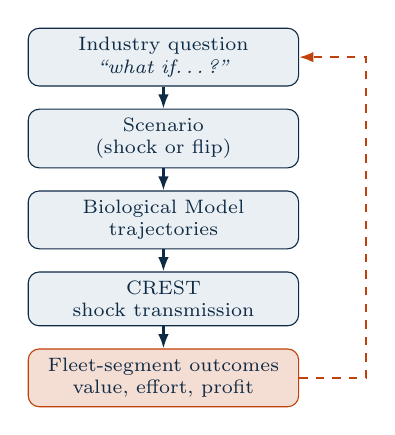
\begin{tikzpicture}[
          node distance=2.8mm and 3mm,
          box/.style={draw=bimnavy, rounded corners, fill=bimsteel!12,
                      align=center, minimum height=5.5mm, text width=3.2cm,
                      font=\scriptsize, text=bimnavy},
          outbox/.style={box, fill=bimorange!18, draw=bimorange},
          arr/.style={-{Latex[length=1.8mm]}, thick, bimnavy}
        ]
        \node[box] (q) {Industry question\\\emph{``what if\dots?''}};
        \node[box, below=of q] (s) {Scenario \\ (shock or flip)};
        \node[box, below=of s] (bm) {Biological Model \\ trajectories};
        \node[box, below=of bm] (crest) {CREST \\ shock transmission};
        \node[outbox, below=of crest] (out) {Fleet-segment outcomes \\ value, effort, profit};
        \draw[arr] (q) -- (s);
        \draw[arr] (s) -- (bm);
        \draw[arr] (bm) -- (crest);
        \draw[arr] (crest) -- (out);
        \draw[arr, dashed, bimorange] (out.east) -- ++(0.85,0) |- (q.east);
      \end{tikzpicture}

      \vspace{1mm}
      \footnotesize Outcomes reframe the next question --- resilient, or should it be?\par
    \end{column}
  \end{columns}
\end{frame}

% ============================================================
\section{Expert elicitation}

\begin{frame}{5. Expert --- which uncertainties matter?}
  \begin{columns}[T]
    \begin{column}{0.58\textwidth}
      \begin{itemize}
        \item Scoping \emph{which} shocks are worth testing is a formal step --- structured elicitation, not only an analyst's list
        \item Precedent (Eastern Atlantic bluefin, ICCAT/GBYP): uncertainties scored for \emph{importance}, \emph{knowledge} and \emph{representation} (Leach et al., 2014)
        \item That prioritisation feeds CREST scenario design
        \item Policy response: insurance / mutual funds to mediate revenue shocks (Mumford et al., 2009)
      \end{itemize}
    \end{column}
    \begin{column}{0.38\textwidth}
      \centering
      \textbf{Elicitation dimensions}
      \begin{itemize}
        \item Importance --- impact on objectives
        \item Knowledge --- reducible by research?
        \item Representation --- in the assessment?
      \end{itemize}
      \vspace{3mm}
      \textbf{Closing thread}
      \begin{itemize}
        \item Advice conditions on the past
        \item Scenarios probe flips ahead
        \item CREST asks: is the fleet ready?
      \end{itemize}
    \end{column}
  \end{columns}
\end{frame}

\begin{frame}{References}
  \footnotesize
  \begin{itemize}
    \item Kell, L.T. (2026). \textit{Simulation of future TACs}, draft chapter, BIM Resilience report.
    \item Mumford, J.D., Leach, A.W., Levontin, P., Kell, L.T. (2009). Insurance mechanisms to mediate economic risks in marine fisheries. \textit{ICES J.\ Mar.\ Sci.}, 66, 950--959. \url{https://doi.org/10.1093/icesjms/fsp100}
    \item Leach, A.W.\ et al.\ (2014). Identification and prioritization of uncertainties for management of Eastern Atlantic bluefin tuna. \textit{Marine Policy}, 48, 84--92. \url{https://doi.org/10.1016/j.marpol.2014.03.010}
  \end{itemize}
\end{frame}

\end{document}
